Robot localization a major problem in mobile robotics. Robot must know its location in an environment for real time applications. The challenge is that robot determines its pose from some internal sensors like wheel encoders, \acrshort{lidar}, \acrshort{gps}, \acrshort{imu}, camera. which always consists some noise. An accurate robot positioning is a fundamental challenge. Camera based Odometry is a novel technique which allows a robot to localize accurately by using sequential images captured by a camera attached to it. This section serves basics of Visual Odometry, different \acrshort{vo} approaches and state of the art \acrshort{vo} methods.\\
\begin{figure}[h]
	\centering
	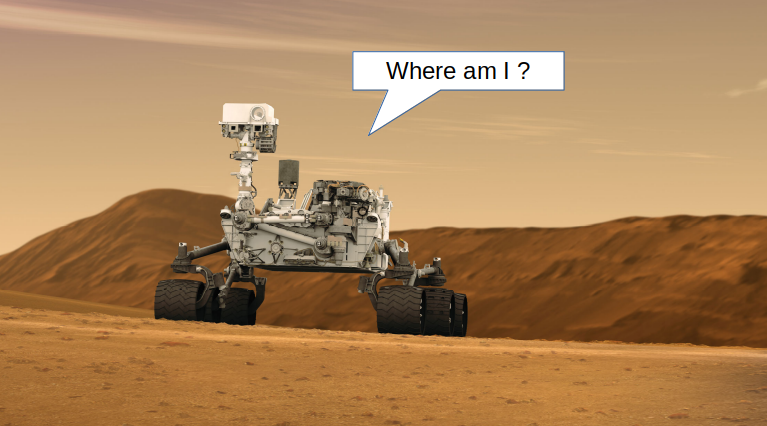
\includegraphics[width=0.9\textwidth]{where_am_i}
	\caption{NASA Path finder robot\cite{nasa}}
\end{figure}
\section{Basics}
According to Khalid Yousif et al.\cite{KhalidYousif-et-al-2015} \acrshort{vo} is defined as "the process of estimating the egomotion (translation and rotation with respect to a reference frame) of an agent(e.g. vehicle, human and robot) by observing a sequence of images using single or multiple cameras attached to it". Structure From Motion (SFM) is a method in computer vision which produces 3D reconstruction of environment and camera poses from set of images \cite{ScaramuzzaVO}. \acrshort{vo} focuses on 3D motion of the camera sequentially in real time which is also known as Sequential \acrshort{sfm} in computer vision. \acrshort{vo} focuses on local mapping and incrementally estimate the camera trajectory and performs local optimization whereas \acrshort{slam} performs localization and global mapping simultaneously.

\subsection{Visual Odometry Pipeline}
\acrshort{vo} pipeline is summarized in Figure \ref{fig:flow}. For every image frame (or image pair for stereo case) 2D features are detected. Feature detection finds 2D features like corners, edges, blobs etc. Next comes feature matching, it will find same features in previous images and reprojects on those images. The matched features are known as image correspondences which are tracked using local search methods, such as correlation. The next step consists of computing relative motion between two images in particular time. There are three different approaches for motion estimation depending on the correspondences specified in 3D or 2D. Global camera pose is determined by concatenation of the previous camera pose. Finally, an iterative local optimization known as \acrshort{ba} can be done over some previous image frames to obtain a more accurate estimate of the local trajectory.
\begin{figure}[h]
	\centering
	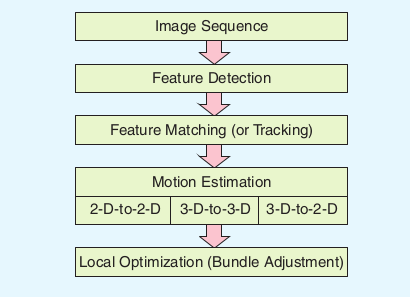
\includegraphics[width=1.0\textwidth]{vo_pipeline}
	\caption{Visual Odometry Pipeline}
	\label{fig:flow}
\end{figure}
\section{Types of Visual Odometry}
\label{section:vo_types}
\acrshort{vo} is mainly classified based on types of camera used for such as stereo, monocular, omnidirectional, and RGB-D cameras. Monocular \acrshort{vo} suffers from scale ambiguity because of unknown depth information of images. Stereo \acrshort{vo} solves this scaling problem by retrieving depth information using two cameras at little on distance known as baseline. Stereo case can be degraded to monocular if the baseline (distance between two image sensors) is much smaller than distances to scene from the camera.\\
\newline
These methods are further classified according to their approach as Indirect (Feature based), Direct (Appearance based) and Hybrid Approach (mixture of both approaches).

\subsection{Indirect Approach}
This is a classical approach for \acrshort{vo} and \acrshort{sfm}. Indirect or Feature-based method involves extraction of some features such as corners, edges etc. from image frames as seen in figure \ref{fig:feature}. These features are then matched and tracked in two consecutive image frames. Based on the feature tracking motion of camera is estimated. This approach can typically divided into two steps 1. Feature detection and matching, 2. Geometric optimization on the computed point correspondences. In first step an image is matched with a previous image by comparing each feature in both images and calculating euclidean distance of feature vectors to find candidate matching features\cite{Aqel-et-al-2016}. In second step using these match correspondences the camera motion and surrounding 3D geometry can be estimated. In case of stereo \acrshort{vo} the features are first compared with each image pair and thus depth information of feature can be estimated. In this approach the reprojection error is minimized using Bundle Adjustment because keypoints positions (geometric quantities) are used to determine camera pose. Bundle adjustment problem is described as below. 
\begin{equation*}
	T_{k,k-1} = arg min_{T} \sum_{i} \| u^{'}_{i}- u_{i}\|^{2}_{\Sigma}
\end{equation*}
where   $u^{'}_{i} = \pi (P_{i},T_{k,k-1})$ , $ u_{i} $ is $ i^{th} $  pixel 2D positions and $ u^{'}_{i} $ is reprojected 2D pixel position using 3D projection $(\pi)$.  
\newline
\begin{figure}[h]
	\centering
	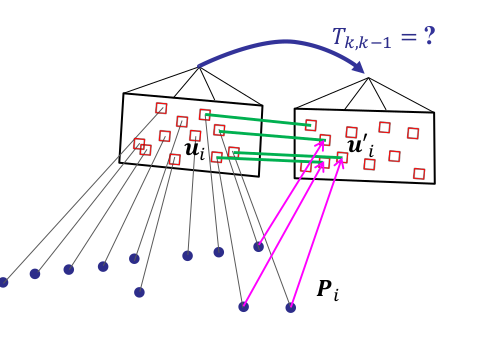
\includegraphics[width=0.8\textwidth]{indirect}
	\caption{Indirect method Optimizes Reprojection Error \cite{lecture}}
	\label{fig:feature}
\end{figure}
\\
The disadvantage of feature-based approaches is their low speed due to feature extraction and matching at every frame, the necessity for robust estimation techniques that deal with erroneous correspondences (e.g. \acrshort{ransac}) and the fact that most feature detectors are optimized for speed rather than precision \cite{7782863}.

\subsection{Direct Approach}
\label{direct}
Direct methods use pixel intensity as an information instead of extracting features and tracking them for motion estimation. Direct methods are based on assumption that brightness remains constant in all image frames \cite{Irani-et-al-1999}. Direct methods are also known as Appearance based methods as they monitor intensity of image pixels in consecutive images. Camera pose is estimated by optical-flow algorithms which determine the displacement of brightness in a group of pixels using intensity values from one image to another \cite{Aqel-et-al-2016}. Two types of such algorithms exist known as Dense and Sparse optical-flow methods. Dense approach is less robust to noise as compared to other. Sparse methods use only those features which have more variance than others in \acrshort{roi}. One of the most used sparse based algorithm for tracking is Lucas-Kanade method \cite{Lucas81}. As there is no feature extraction step is involved direct approach minimizes directly the photometric error as seen in figure \ref{fig:direct}. The mathematical problem can be formulated as below. 
\begin{equation*}
	T_{k,k-1} = arg min_{T} \sum_{i} \| I_{k}(u^{'}_{i})- I_{k-1}(u_{i})\|^{2}_{\sigma}
\end{equation*}
where $u^{'}_{i} = \pi (P_{i},T_{k,k-1})$ and $I_{k} $ is  $k_{th}$ image.
\newline
\begin{figure}[h]
	\centering
	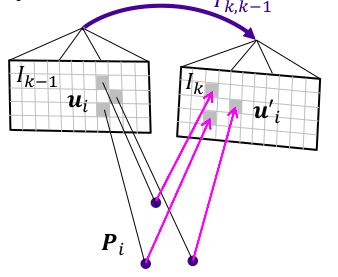
\includegraphics[width=0.8\textwidth]{direct}
	\caption{Direct Method Optimizes Photometric Error \cite{lecture}}
	\label{fig:direct}
\end{figure}
\\ 
Depending upon the number of feature selection for calculating 3D geometry Direct methods can be divided into three types such as Dense, Semi-dense and Sparse methods. A graphical overview of these methods can be seen in figure \ref{fig:dense_sparse}. Dense approaches use every pixel in the image, where as semi-dense use just the pixels with high intensity gradient and sparse approach uses selected pixels at corners or along intensity gradient edges \cite{engel14eccv}.
\newline
\begin{figure}[h]
	\centering
	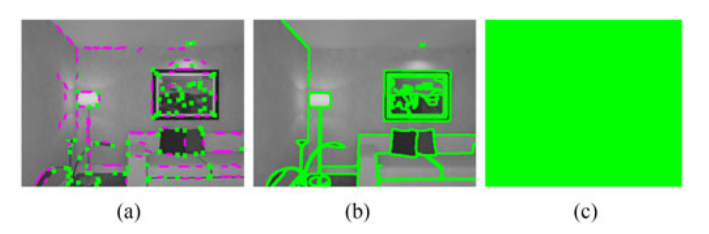
\includegraphics[scale=0.6]{dense_sparse}
	\caption{Image-to-model alignment (marked in green for corners and magenta for
		edgelets) for sparse, semi-dense, and dense methods \cite{7782863}.}
	\label{fig:dense_sparse}
\end{figure}
\\
As Direct methods minimize the photometric error (intensity difference) for tracking between two images they require a well calibrated camera as compared to Indirect methods because they minimize the image pixel positions on images. A simple process comparison is described in the Figure.\ref{fig:direct_indirect}. Indirect methods have been very popular for a long time but recent advances in direct methods have shown better accuracy and robustness, especially when the images do not contain enough explicit corner features \cite{Engel-et-al-pami2018}. The robustness in direct approach comes from the joint estimation of motion and correspondences as well as the ability to also use non-corner pixels, corresponding to edges or even smooth image regions\cite{gao2018ldso}.
\begin{figure}[h]
	\centering
	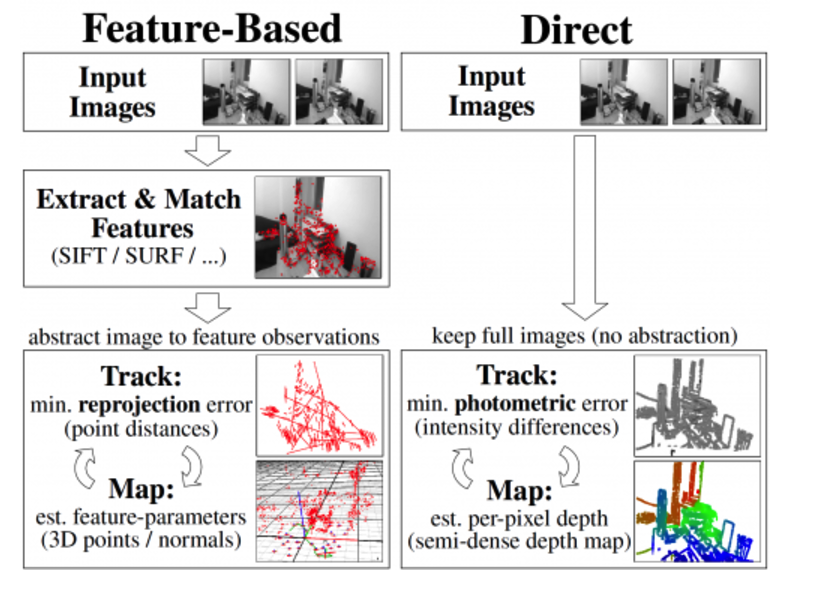
\includegraphics[width=1.0\textwidth]{direct_indirect}
	\caption{Process comparison between Direct and Indirect methods \cite{engel14eccv}.}
	\label{fig:direct_indirect}
\end{figure}
\subsection{Hybrid Approach}
Indirect approach fails to deal with texture-less or low-textured environments of a single pattern such as sandy soil, asphalt and concrete. Lesser number of features detected in these types of environments make this approach inefficient. The direct approaches are more robust and accurate than indirect approach in low-textured or symmetric environment but they are not much robust to image occlusions or inconsistencies in system (e.g rolling shutter). To have a advantages of both approaches the best solution is to use the combination of both approaches which combines tracking of salient features over frames and use the pixel intensity as an information \cite{Aqel-et-al-2016}. Forster et al.\cite{7782863} proposed a hybrid approach in which they use a 4x4 patch around features and estimate the camera pose by minimizing the photometric error of these patches. For pose and structure refinement, the reprojection error of every feature is calculated with respect to the nearest key-frame that has observed the feature at nearly the same angle.

\subsection{Monocular vs Stereo}
In Monocular \acrshort{vo}, a single camera is used for the whole pipeline. In this case features need to be observed in subsequent frames in order to track motion properly. Features observed in the first frame are triangulated into 3D points with help of second frame, and then transformation can be calculated using third frame \cite{KhalidYousif-et-al-2015}. While in stereo case, 3D points can be reconstructed (by triangulation) only by observing the features in left and right images of a single pair simultaneously. Motion is estimated by observing features in two successive frames (both left and right). Stereo approach has an advantage of depth information of environment because it can obtain the disparity in scene. Where as monocular cameras can measure motion using pixel information only with no knowledge of scene depth. When the distance between scene to stereo camera becomes very long compared to the baseline (distance between left and right camera), the stereo case can be degraded to monocular because its very erroneous to measure the depth for far scene. 

\section{State of the Art}
\acrshort{vo} has been very active research topic in recent years. There has been many algorithms published based on the approaches discussed in section \ref{section:vo_types} and research is still ongoing. There are several papers published on current state of \acrshort{vo}. They are \cite{Aqel-et-al-2016}, \cite{KhalidYousif-et-al-2015} ,\cite{ScaramuzzaVO}. Currently research is focused based on the deep learning methods \cite{7989236}, \cite{yang20d3vo} which is not in the scope of this thesis. Though \acrshort{vo} and \acrshort{v-slam} are widely researched topics it is still difficult to get an overview of all the algorithms. A list of various \acrshort{vo} and \acrshort{v-slam} algorithms, references and code if available can be found at \ref{section:A.1}. This list is referred from \cite{chris}. The list presents mostly all algorithms invented so far using cameras. Also, these algorithms can be classified according to their approaches. Considering these facts and other criteria such as
\begin{enumerate}
	\item runs on CPU 
	\item open source availability 
	\item real-time performance
	\item works for monocular sensor
	\item state of the art
\end{enumerate}	
three algorithms (one from each approach discussed in section \ref{section:vo_types})
\begin{enumerate}
    \item \acrshort{orb} \acrshort{slam} \cite{Mur-Artal} 
    \item Direct Sparse Odometry with Loop closure (LDSO)\cite{gao2018ldso} 
  	\item Semi-direct Visual Odometry (SVO) \cite{7782863} 
\end{enumerate}	     
are selected for implementation and later evaluation. In the next section these three algorithms their approaches, pros and cons compared to each other are described.

\subsection{ORB-SLAM}
\acrshort{orb} \acrshort{slam} is a very popular feature(Indirect) based visual \acrshort{slam} approach. It uses an open-source \acrshort{orb} feature descriptors as feature extraction and matching, which was developed by Rublee et al.\cite{ORB}. These \acrshort{orb} features are robust to rotation, scale and also provides good invariance to auto-exposure and illumination changes. Further more they are fast to extract and match which makes them suitable for real-time applications\cite{Mur-Artal}. Mur-Artal et al. \cite{Mur-Artal} used an approach of parallel threads for \acrshort{orb}\acrshort{slam} similar to that of used in \acrshort{ptam} \cite{4538852}. It has mainly three parallel threads 1.Tracking, 2.Local Mapping and 3.Loop Closing. Loop closing is the thread of performing Global \acrshort{ba}. This section describes the working of all modules. A detailed approach is given in the figure \ref{fig:orbslam}.
\begin{figure}[h]
	\centering
	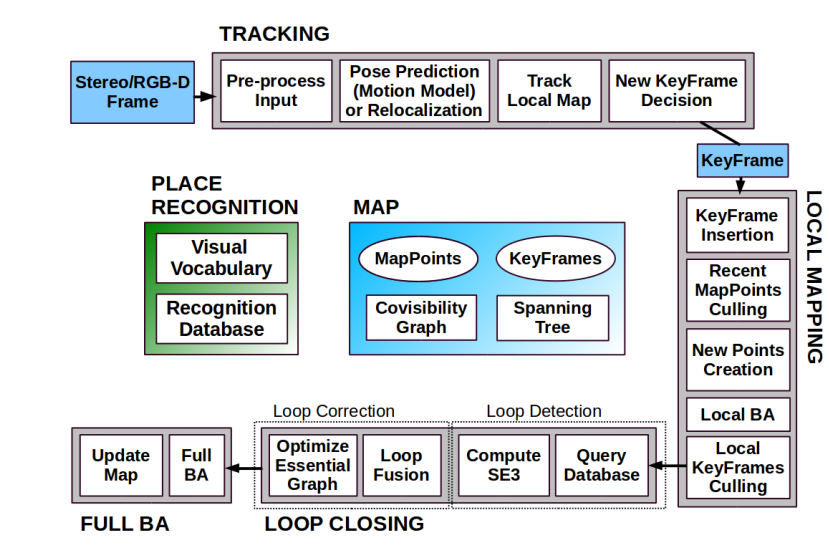
\includegraphics[width=1.0\textwidth]{orbslam}
	\caption{A process overview of ORB-SLAM \cite{Mur-Artal}}
	\label{fig:orbslam}
\end{figure}
\newline
\acrshort{orb} \acrshort{slam} consists mainly five modules :
\begin{enumerate}
	\item Feature extraction 
	\item Initialization
	\item Tracking
	\item Local mapping
	\item Loop closing
\end{enumerate}	

\subsubsection{Feature Extraction}
The feature extraction module takes every image as input. Images are first blurred and then used to create a layer of an image pyramid with pre-defined scale factor (e.g, 1.2) up to 8 levels and added on top of the image. As \acrshort{orb} \acrshort{slam} uses the Features from Accelerated Segment Test (\acrshort{fast}) for feature extraction, it might lose some features at only one scale level. A working principle of \acrshort{fast} detector is shown in figure \ref{fig:fast}. Then according to image resolution \acrshort{fast} corners are extracted for initial detector threshold of 20. If number of corners are not enough then threshold further reduced to 7 and again corners are detected. To have a homogeneous distribution images is divided into equal size fo grids until each grid has a pre-defined minimum number of corners (e.g. 5). After this step only the corner with highest score in each grid are kept and other are discarded. \\
\linebreak
Next step is to compute the Oriented Fast and Rotated Brief \acrshort{orb} feature descriptor, an extension and combined of \acrshort{fast} and \acrshort{brief}. The working of it explained here \cite{ORB}. The All features are undistorted using already provided camera calibration data from setting file. These \acrshort{orb} descriptors are further used in the feature matching step.
\begin{figure}[h]
	\centering
	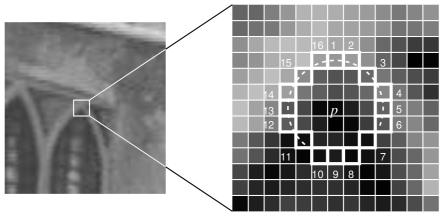
\includegraphics[width=0.8\textwidth]{fast}
	\caption{\acrshort{fast} corner detection principle. For every pixel {p} a circle with
		a radius of three pixels around it considered. A corner is detected if at minimum nine neighboring pixels in circle are either brighter or darker than {p} \cite{fast}.}
	\label{fig:fast}
\end{figure}

\subsubsection{Initialization}
\acrshort{orb} \acrshort{slam} requires strong initialization because the features tracked in this module are also used to initialize 3D map. Number of feature extracted from two frames should be at least 100 to start this module. After initialization the current frame is used to match the features with initial frame. In this module feature matching is done by comparing the descriptor distance and orientation of 2D features of current frame with that of initial frame.\\
\linebreak
For every feature in first frame a small region (e.g 200 x 200 pixels) around this feature is selected in current frame. Every image is divided into sufficient amount of grid cell according the image resolution. For example the image resolution of one of the camera used in this thesis is 1024 x 1024. And the grid is divided into cells with 64 columns and 64 rows. Then distance to the feature with all features in that cell of current frame is computed. If distance is less than 50 and the shortest distance is 0.9 of second shortest distance then it passed to the orientation check. For orientation test all matches are sorted into 12 equally angled bins. If the orientation is with in limit of the one neighboring bin from each side then it is considered as a match. For further processing minimum number of matches should be found. Authors have set default as 100 in code but it can be vary according to the scene). \\
\linebreak
After successful matching, tt computes possibility of homography and fundamental matrix in parallel threads. Homography relates the mapping of two projection of a planer scene. The concept is shown in figure \ref{fig:h} The mathematical formula for homography is:
\begin{equation*}
    x^{'}_{i} = Hx_{i}    
\end{equation*}    
    $  x_{i} \in  \mathbb{R}^{3} $    Homogeneous pixel coordinates in first frame \\ 
    $  x{'}_{i} \in  \mathbb{R}^{3} $    Homogeneous pixel coordinates in second frame\\ 
    H  = homography matrix \\
\newline
\begin{figure}[h]
	\centering
	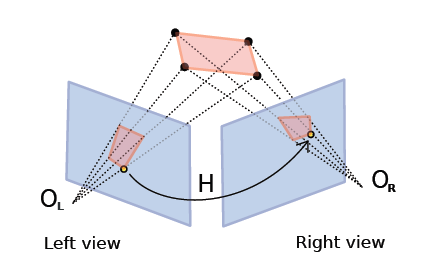
\includegraphics[width=0.7\textwidth]{Homo}
	\caption{Homography matrix H maps image points of a scene plane seen from one coordinate frame system $ O_{L} $ to the corresponding system $ O_{R} $ \cite{multiview}.}
	\label{fig:h}
\end{figure}
\\
The fundamental matrix (F) is a relation between two images viewing the same scene where those point’s projections are visible in the stereo image pairs. The figure \ref{fig:F} describes the epipolar geometry of a scene. The further details on epipolar geometry can be found in \cite{multiview_geometry}. Given a point correspondence between two views 
$ (x_{i} , x{'}_{i}) $ the relation for F is : 
\begin{equation*}
x^{'T}_{i}Fx_{i} = 0    
\end{equation*}    
\newline
\begin{figure}[h]
	\centering
	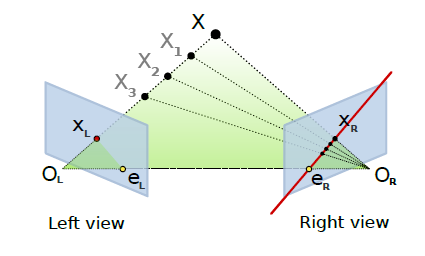
\includegraphics[width=0.7\textwidth]{Funda}
	\caption{The Epipolar geometry has constraint that given a projection $ x_{L} $ in one image the corresponding point $ x_{R} $ in the other image has to lie on the line $ Fx_{i} $ \cite{multiview}.}
	\label{fig:F}
\end{figure}
\\
These both models are computed within \acrshort{ransac} with same number of iterations and then model score (sum of reprojection errors) is calculated by reprojection for each model.
The decision of which model to use is decided by computing heuristic defined as : 

\begin{equation*}
R_{H} = S_{H} / {S_{H} + S_{F}}  
\end{equation*}  
\\ 
where $ R_{H} $ is Heuristic, $ S_{H} $ is Homography score and $ S_{F} $ is Fundamental Matrix score \\
\linebreak
If $ R_{H}  > 0.40 $ homography is chosen for pose estimation, otherwise fundamental matrix. 
Total 8 motion hypothesis can be recovered in case of homography where as in case of fundamental matrix 4 motion hypothesis can be recovered as explained in \cite{multiview_geometry}. Each hypothesis is checked by triangulating all matches using Direct Linear Transformation (DLT) algorithm \cite{multiview_geometry} and checked whether they lie in front of camera. The one with big enough parallax and small reprojection error is selected. In last step minimum parallax is set to one degree and minimum 90 percent of total matches needs to be correctly triangulated. \\
\linebreak
After acceptance of these step an initial map is created using the triangulated matches as map points and both frames as keyframes and a global \acrshort{ba} is run on this map. At least 100 map points should be created after this step otherwise initialization will be discarded and the whole process will be repeated until successful initialization. 

\subsubsection{Tracking}
After successful initialization tracking comes into picture to estimate the camera motion.
Tracking is mainly divided into two parts. The first part can be done by two ways depending on existence of motion model. As this algorithm uses constant motion model for tracking it simply assumes that the camera will move with constant velocity in next frames also which makes this approach more simple. \\
\linebreak
If constant motion model exist the tracking module run feature matching algorithm by assuming that map points in previous frame can be found within certain region in the next frame based on camera velocity. The size of region depends on the scale pyramid in which the features are extracted (e.g for base scale it will be 14 x 14 pixels). With given threshold if number of matches found are less than 20 then it will again search with wider window of 28 x 28 pixels. Even if there are less than 15 matches found then motion model will fail and 
tracking will be run without using motion model.\\
\linebreak
If motion model is failed then it takes a different approach of tracking. In this approach instead of projecting features they are transformed into bag of visual words vector and compared with the reference keyframe. For this purpose \acrshort{orb} \acrshort{slam} uses the DBoW2 library developed by Gálves-López and Tardós \cite{DboW}. \\
\linebreak
DBoW2 creates a database of bag of words vectors. The query frame's features descriptors are compared with the tree nodes in DBoW2 and it will determine how each word occurs in every image. By creating the bag of words vector in every image it can simply be compared with other images by taking $ L_{1} $ norm of two vectors $ v_{1} $ and $ v_{2} $  as per below equation. \\

\begin{equation*}
s(v_{1},v_{2}) = 1 - \frac{1}{2} \arrowvert \frac{v_{1}}{|v_{1}|} - \frac{v_{2}}{|v_{2}|} \arrowvert 
\label{norm}
\end{equation*}  
\linebreak 
Tracking module uses this database to compare the features in current frame with reference keyframe. Feature with lowest hamming distance with given threshold is found. If matches are not more 15 tracking will be aborted and relocalization module will be triggered. If one of these approach run successful with minimum matches then these matches will be optimized using previously assumed pose. The pose optimization is done using $ g^{2}o $ library \cite{g2o}. \\
\linebreak
If first part is succeeded, then second part of tracking local map comes into picture. To reduce the processing time \acrshort{orb} \acrshort{slam} keeps a local map with only a set of keyframes $ k_{1} $ that share map points with current frame and another set $k_{2} $ with neighbors to the $ k_{1} $ in covisibility graph. A reference frame for a local map and current frame is created which shares most map points with the current frame. For every map point seen in $ k_{1} $ and $ k_{2} $ is searched in current frame as mentioned in \cite{orbslam} follows the below procedure: 
\begin{enumerate}
	\item Project the map point in the current frame. Keep it if its inside image otherwise discard.
	\item Compute the angle between the current viewing ray v and the map point mean viewing
	direction n. Discard if v · n < cos(60°).
	\item Determine the distance d from map point to camera center. check the limit of scale invariance the map point $ d \notin [d_ {min} , d_{max}] $. 
	\item Compute the scale level in the frame by taking ratio $ d/d_{min} $.
	\item Compare the representative descriptor D of the map point with the unmatched features in the current frame, at the predicted scale, and near the projection and associate the map point with the best match.
\end{enumerate}
After all map points are processed, the camera pose is optimized again using these matched points and keep the pose if minimum matches stays 30 otherwise tracking will be lost and relocalization will be triggered. For fresh relocalization the minimum matches required are 50. \\
\newline
The last part of tracking is whether to mark the current frame as keyframe or not. There are four conditions which should be satisfy:
\begin{enumerate}
	\item The last relocalization must have happened before 20 frames ago.
	\item Local mapping thread is idle or more than 20 frames have passed since last keyframe insertion.
	\item The current frame tracks minimum 50 points.
	\item The current frame tracks less than 90\% of the points than reference keyframe (last keyframe).
\end{enumerate}
These conditions ensure good relocalization, stopping local \acrshort{ba}, good tracking and minimum visual change respectively. With this tracking module ends. 

\subsubsection{Local Mapping} 
Local mapping is independent thread running in its own when new map points and keyframe is inserted. This module takes care of all local map points and keyframes and keeps them up to date by constantly pose optimizing. The module run in loop where it gets updated ever 3 ms whether there is any new keyframe is inserted in local map. After getting key frames it follows the below steps: 
\begin{enumerate}
	\item Integration fo new keyframe into local map and update all connections. 
	\item Check conditions for map points deletion (actually not deleted rather unused). Map point will be removed if: 
	   \begin{enumerate}
		\item Its ratio of visibility frequency and matching frequency is less than 0.25
		\item It has matched less than three times and more than one keyframe has been added since the point insertion in local map.
	   \end{enumerate}
	\item New points are created by triangulating the matched features of new keyframe with that of connected keyframes(20 such keyframes which share most map points with current keyframe).  
	\item If no new keyframe is in waiting then fuse the duplicate map points.
	\item Perform a local \acrshort{ba} and remove those keyframes which shares at least 90\% of map points with minimum three keyframes. If there is new keyframe inserted in loop during local \acrshort{ba} then stop it and include the keyframe first.
\end{enumerate}

\subsubsection{Loop Closing} 
Loop closing is also an independent thread which run in its own. Loop closing will observe the data and triggers if it detect loop. This module can be divided in three parts:
\begin{enumerate}
	\item Loop detection
	\item Loop confirmation
	\item Loop correction or refinement
\end{enumerate}
Loop detection behaves like local mapping that it triggers when a new keyframe is available. After receiving new keyframe it will look for connected frames in its covisibility graph.
For every keyframes it will compute the score as per equation \ref{norm}. If there is minimum 10 keyframes in the map and last loop closing has done before 10 keyframes ago then it will pose a query to keyframe database and check for at least one bag of word with current keyframe with the highest score of than minimum of calculated those of all. All keyframes are then added to the loop closing candidates. An explanation can be found in \cite{chris}.\\
\newline
After having enough loop candidates, the last keyframe from candidates id used to check whether it can be considered as a loop. \acrshort{orb} \acrshort{slam} uses the same method that was used in tracking module for track without motion model. However, instead to matching between 2D and 3D points here it will look for matching between 3D map points seen in current keyframe directly to that of in candidate frame by means of \acrshort{orb} descriptors. Confirmation requires at least 20 matches. However due to drift accumulation these match map points are not likely be close to the each others. An example of this illustrated in the figure \ref{fig:loop}.\\
\newline In general, localization has six degree of freedom (3-rotational and 3-translational) which accumulate the drift. However, monocular case suffers from scale-drift in addition to those six. Single camera can not sense the depth of scene much like humans when try to see with one eye only. It can not differentiate between an real size structure and its 3D miniature.
This situation is further discussed in later section. \acrshort{orb} \acrshort{slam} can recover the scale drift up tom some level by estimating the similarity transformation between current and candidate keyframe. A similarity transformation can be structure as follows:
\begin{equation*}
S = 
\begin{bmatrix}
sR & t \\
0 & 1
\end{bmatrix}
\label{similarity}
\end{equation*} 
with,\\
$ S \in Sim(3)$  \ \ Similarity transformation \\
$ s \in \mathbb{R}$ \ \ \ \ \ \ \ \ \ \ Scale factor \\
$ R \in SO(3) $  \ \ \   Rotation matrix \\
$ t \in \mathbb{R^{3}} $ \ \ \ \ \ \ \ \ \ Translation vector
\begin{figure}[H]
	\centering
	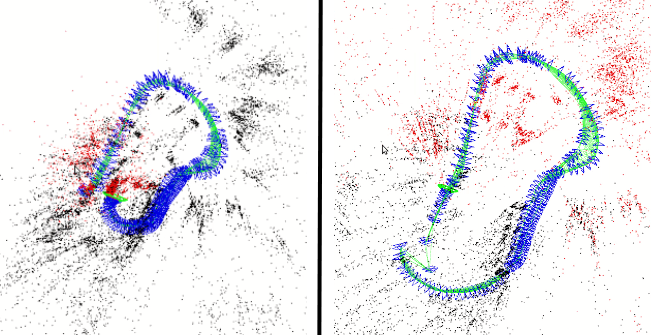
\includegraphics[width=1.0\textwidth]{loop}
	\caption{\acrshort{orb} \acrshort{slam} mapping result showing of one of the sequences in this thesis work. left and right images show the camera trajectory just before finding loop and after loop closing respectively.}
	\label{fig:loop}
\end{figure}
\noindent Equation \ref{similarity} is solved by method of Horn described in. Using this transformation it will again search for more matches of 3D points to further optimize the transformation S. If at least 20 matches found then last check for candidate frame is to search for more matches by projecting map points found in all connected keyframes. Minimum 40 matches required to finally accept the candidate and perform the last step(loop refinement) of this module. \\
\newline 
Once loop is accepted the last step is to refine the loop. During this step the local mapping is interrupted and pose optimization stops. In covisibility graph current keyframe is connected to those which are around to the candidate keyframe. Then it collects all keyframes and corrects their pose along with map points using the calculated similarity transformation which will move the all keyframes and map points connected to current keyframe. At this point covisibility graph get updated with those connections. After this step the keyframes not connected to current keyframe needs to be corrected. Also, there will be some duplicate map points in connected keyframes which can be found by projecting them into 2D image coordinates and matching with features. If match is found with already linked map point then that will be removed due to duplication \\
\newline 
In next step the correction will propagate over the essential graph, see figure \ref{fig:orbslam}. It will make optimization more focused and quicker. The optimization on Sim(3) constraints is explained in \cite{Mur-Artal}. The final step is to perform global \acrshort{ba}. It will run in separate thread and optimizes all keyframes and map points. As stated in \cite{Mur-Artal} this is very costly step. There is also problem of merging the optimized pose with the current map because map keeps changing while global \acrshort{ba} is performing. Therefore \acrshort{ba} has to update those frames also which are not yet in the \acrshort{ba}. These keyframes can be updated by the transformation of their parent keyframe in the spanning tree.

\subsubsection{Bundle Adjustment}
This section explains the working of Bundle Adjustment. \acrshort{ba} is well-known algorithm used in graph based \acrshort{slam} methods. Ideally a projection of 3D point X to its 2D point x should follow as per x = PX with P being the camera matrix consisting extrinsic and intrinsic parameters. However in real camera is subjected to noise which may not fulfill this relation. In case of multiple cameras or views this situation can be illustrated as in figure \ref{fig:ba}. The goal of \acrshort{ba} is to correctly estimate the camera projection matrices($ P^{i}$) and 3D points($X^{j}$) and their corresponding 2D image points($ x_{i}^{j} $) which satisfy:
\begin{equation*}
 x_{i}^{j} = P^{i}X^{j}
\end{equation*} 
With simultaneously minimizing the reprojection error between reprojected point and the corresponding image point for every frame it is visible in \cite{multiview_geometry}. \acrshort{ba} assumes the noise to be Gaussian. The \acrshort{ba} minimizes reprojection error:
\begin{equation*}
 min_{P^{i},X_{j}} \sum_{ij} d(P^{i}X_{j},x_{j}^{i})^{2}
\end{equation*} 
with d(x,y) image pixel distance between homogeneous points x and y. \\
\newline 
As number of unknowns increase it becomes difficult to solve. For example, with m views and n points it needs to find a solution for 3n+11m unknowns as camera matrix P has 11 degrees of freedom.

\begin{figure}[h]
	\centering
	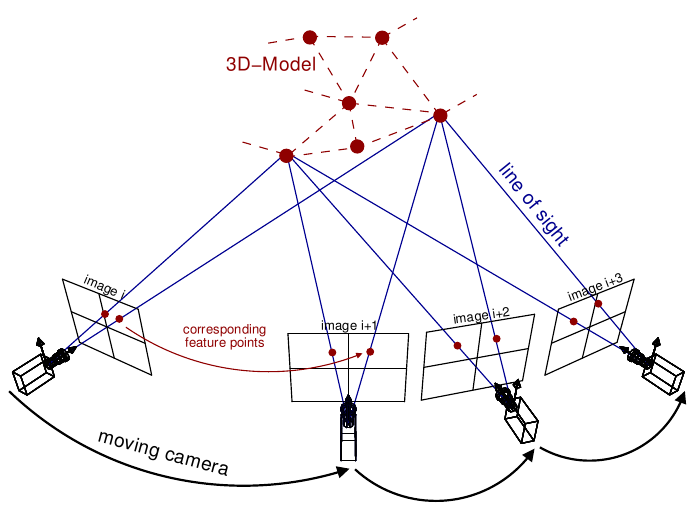
\includegraphics[width=0.9\textwidth]{ba}
	\caption{An illustration of \acrshort{ba} with multiple cameras seeing same scene \cite{sfm}.}
	\label{fig:ba}
\end{figure}

\subsection{Direct Sparse Odometry with Loop Closure (LDSO)}
DSO (Direct Sparse Odometry) is one of the few \acrshort{vo} which uses fully Direct approach. It is developed by Dr. Jakob Engel in 2016 at Cremer's lab, Technical University of Munich.
\acrshort{dso} is not a complete \acrshort{slam} system while an extended version of \acrshort{dso} which is known as \acrshort{ldso} \cite{gao2018ldso} comprises of loop closure. 
A main advantage of direct method is that it doesn't require any matched point for motion tracking instead it can make use of any information even plain texture-less surface. In \acrshort{dso} 3D point is derived from the host frame and is multiplied by the depth value and reprojected to all active frames and creates reprojection residuals. A process overview of \acrshort{ldso} can be seen in figure \ref{fig:ldso}. \acrshort{ldso} consists three main modules 
\begin{enumerate}
	\item Tracking(front-end)
	\item Optimization(back-end)
	\item Loop Closure
\end{enumerate}
\begin{figure}[h!]
	\centering
	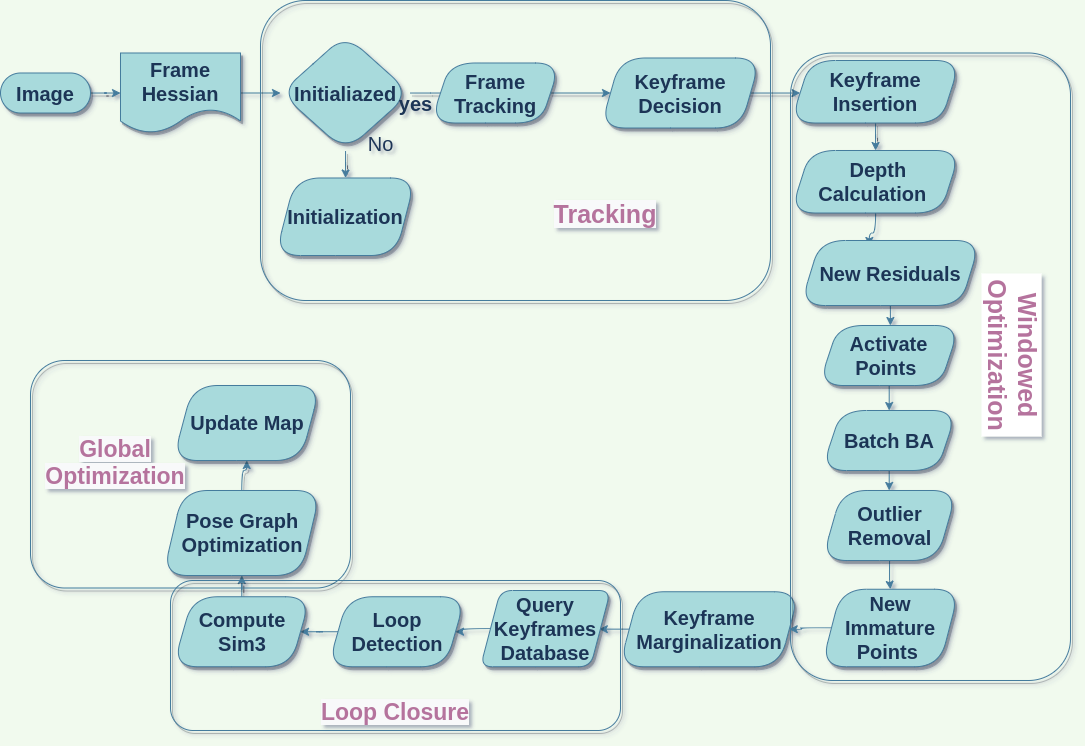
\includegraphics[width=1.0\textwidth]{ldso}
	\caption{Process overview of \acrshort{ldso}}
	\label{fig:ldso}
\end{figure}
\subsubsection{Tracking}
Tracking is main module in \acrshort{dso} which acts as a front-end pipeline. It includes various sub-tasks such as initialization, keyframe creation and marginalization, creation of residuals and points activation. It starts with initialization where all active points are projected onto a new keyframe and creates a semi-dense depth map. Further next frames are tracked with respect to this keyframe using two frame direct image alignment. A multi-scale image pyramid is created for initialization. If \acrshort{rmse} for a frame is more than twice that of the previous frame then direct image alignment is failed and initialization is done using 27 different small rotations in all possible directions. Once initialization is succeed next comes tracking. Frame is A new keyframe is created satisfying following conditions    
\begin{enumerate}
	\item If field of view is changed from last keyframe to current frame then a new keyframe is created. Which can be measure by mean square optical flow (f).
	\item If camera has enough translation creating occlusions of points in frame then a new keyframe is created. It is measured by mean optical flow without considering rotation ($f_{t}$).
	\item If camera exposure time changes above limit then a new keyframe is inserted. Change in exposure time can be measured by relative brightness factor between two frames ($f_{a}$).
\end{enumerate}
Finally, some weighting factors are multiplied with all three criteria and the sum of them is calculated as follows: 
\begin{equation*}
  w_{f} f + w_{ft} f_{t} + w_{fa} f_{a} > T_{kf}
\end{equation*} 
where $w_{f}, w_{ft}, w_{fa} $ are relative weighting factors and $ T_{kf} = 1. $ \\
\newline
After a keyframe is created it is used as host frame and all frames are tracked with respect to it by projecting all immature points onto the host frame. If points have less \acrshort{rmse} then they are converged and inverse depth is estimated for al these points. Next step is to flag keyframes for marginalization. \acrshort{dso} uses sliding window of keyframes for local optimization as show in figure \ref{fig:dso_sliding}. For that it needs to remove older keyframes and others which are not necessary. Marginalization strategy is as follows: 
\begin{enumerate}
	\item Latest two keyframes are always included into sliding window.
	\item Keyframes with less than 5\% of their points visible in latest keyframe are flag as marginalized.  
	\item If active keyframes are more than required then the frames which have more euclidean distance with latest keyframes are marginalized. By doing this more keyframes remains close to the latest frame. 
\end{enumerate}
After flagging keyframes, all active points in the sliding window are projected into a newly created keyframes and new residuals are created using those points. These active points are first selected from all over area of active image frames. The image is divided into 32 x 32 grid.
From every cell, pixels with largest intensity gradient are selected as immature points for further processing. These points are tracked in next frames using discrete search along epipolar line. For a best match depth and associated variance is calculated. Along with this old points are marginalized replacing new candidate points. The number of active points are kept as fixed (e.g. 2000) and distributed equally across all active frames in sliding window. At this points newly created keyframe is optimized using the residuals and the active frames. A batch \acrshort{ba} is used for optimization.  
\begin{figure}[h!]
	\centering
	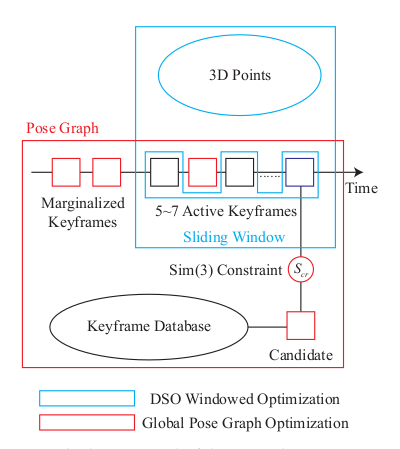
\includegraphics[width=1.0\textwidth]{dso_sliding}
	\caption{Concept of sliding windowed and global pose graph optimization \cite{gao2018ldso}}
	\label{fig:dso_sliding}
\end{figure}
After local optimization next step is outlier removal from the local map. The points which are not tracked along epipolar line and for which photometric error is more than threshold are marked as outliers. For bad frames threshold value is set as higher to avoid all points marked as outliers. After outlier removal new immature points are created using feature detector. These points are used for residual creation. All active frames which are flagged before are marginalized. First all points from respective frame are removed from sliding window and then the frame is marginalized. At this point front-end of \acrshort{dso} is over and further loop closing module starts which is adopted in \acrshort{ldso}.

\subsubsection{Optimization}
Back-end of \acrshort{dso} is very complex module and hard to understand its code. \acrshort{dso} uses Gauss-Newton or Levenberg-Marquardts method for optimization of sliding window \cite{Engel-et-al-pami2018}. The parameters are keyframes and residuals of map points generates the optimization problem. All these terms create a larger linear equation as follow: 
\begin{equation*}
J^{T}WJ\delta x= -J^{T}Wr
\end{equation*} 
Where J ,W,r are Jacobians, weights and residuals respectively, and $ \delta x $ is the overall optimized update. The left side is also known as Hessian matrix (H). This optimization is different that one used in \acrshort{orb}-\acrshort{slam} where it always rebuild the whole optimization problem, solves it and then deconstruct it again. While in \acrshort{dso} this problem is taken as subsequential and the optimization is used as prior for next optimization without destructing it. Hessian matrix has arrow-like famous shape as shown in figure \ref{fig:hessiain}. The sparse structure is advantageous for faster solution of the problem. As geometry in left image is on diagonal it can be solved very efficiently using Schur complement \cite{Engel-et-al-pami2018}. While it becomes harder to solve problem when geometry prior has geometry correlations (right image).   
\begin{figure}[h!]
	\centering
	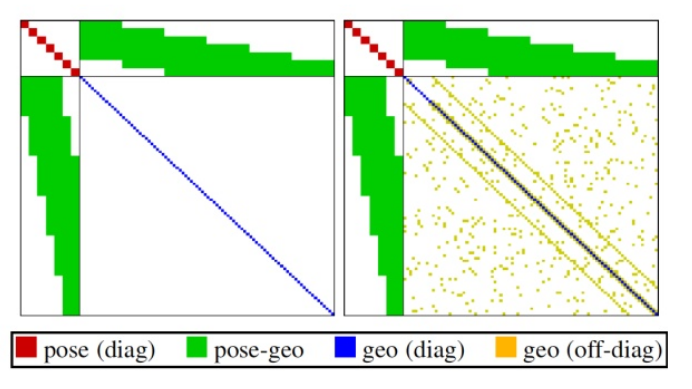
\includegraphics[width=1.0\textwidth]{hessian}
	\caption{Hessian matrix shape in batch \acrshort{ba} \cite{Engel-et-al-pami2018}}
	\label{fig:hessiain}
\end{figure}
\acrshort{dso} \acrshort{ba} is not same as traditional \acrshort{ba} because upper left part is not diagonal matrix rather added by prior camera movement which can be estimated by previous motion status. The priori is generated between the co-visible frames of point when the point is marged and when the frame is marged. \\
\newline
The marginalization is same as discussed in front-end of \acrshort{dso}. A point and frame is marginalized if :
\begin{enumerate}
	\item A point is no longer in field of view of the camera.
	\item Number of keyframes in sliding window exceeded than threshold.  
	\item A frame is marginalized, the map points which use it as host frame will also marginalized.
\end{enumerate}

\subsubsection{Loop Closure}
\acrshort{dso} is pure monocular \acrshort{vo} without global mapping and loop closing functionality. Xinag Gao et al. proposed a loop closing system in \acrshort{dso} \cite{gao2018ldso}. The proposed loop closing is based on pose graph optimization unlike global \acrshort{ba} in \acrshort{orb}-\acrshort{slam}. The figure \ref{fig:dso_sliding} show that while \acrshort{dso} sliding window is working a global pose graph is getting generated using all keyframes including marginalized ones. Reason for \acrshort{ba} would not work for loop closing in \acrshort{dso} is that number of points selected. For this amount of points a photometric \acrshort{ba} is infeasible. One more modification is done in \acrshort{ldso} is that point selection. \acrshort{ldso} along with high gradient pixels corners are also used as features which shows higher repeatability than those high gradient pixels.\\
\newline
Working of loop closing is illustrated in figure \ref{fig:ldso}. First \acrshort{orb} descriptors are computed for each keyframe. A \acrshort{bow} database is built using DBoW \cite{DboW}. All keyframes \acrshort{bow} are stored in a query keyframe database. For every candidate frame its \acrshort{orb} features are matched against the current keyframe. If a loop is detected then the loop correction is started. During this time global map is sate as idle. In loop correction \acrshort{ransac} \acrshort{pnp} is performed to compute an initial SE(3) transformation and if enough number of inliers are found then Sim(3) Pose is calculated using Gauss-Newton by minimizing 3D and 2D geometric constraints \cite{gao2018ldso}. After enough correct local map points pose-graph optimization is done using g2o solver \cite{g2o}. Now the last step in loop closing is fuse the global pose graph with sliding window. In order not to disturb sliding window optimization \acrshort{ldso} update only old poses in the trajectory during loop fusing leaving the current pose as it is. An example of loop closing in \acrshort{ldso} is shown in figure \ref{fig:ldso_loop}. Here the red and yellow lines shows the camera trajectory before and after loop closing. 
\begin{figure}[h!]
	\centering
	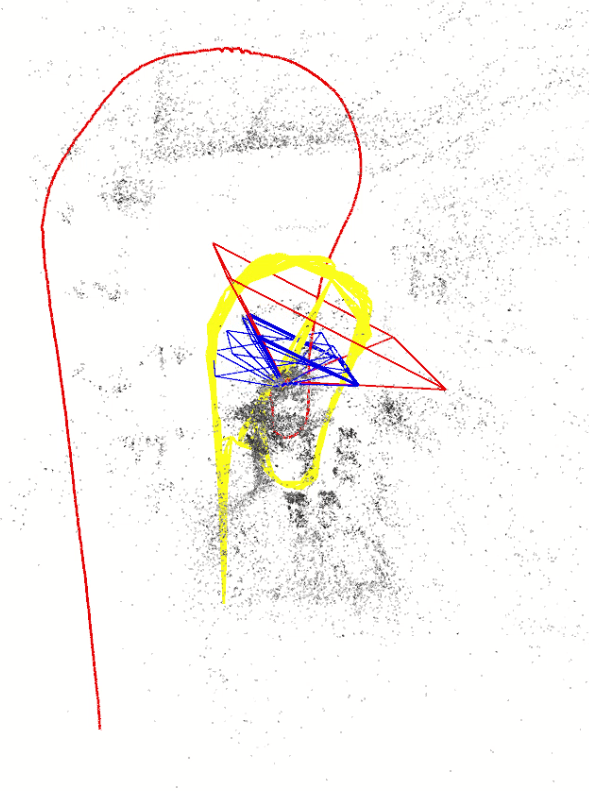
\includegraphics[width=0.5\textwidth]{ldso_loop}
	\caption{Loop closing effect in ldso}
	\label{fig:ldso_loop}
\end{figure}

\subsection{Semi-direct Visual Odometry}
Forster et.al developed first hybrid approach which uses both direct and indirect approaches at different points in the algorithm. They named it as Semi-direct Visual Odometry (SVO). \acrshort{svo} has similarity with \acrshort{ptam} in terms of process as explained in \cite{4538852}. The only difference is that \acrshort{ptam} is fully indirect approach and meant for rather smaller environment while \acrshort{svo} is semi-direct method. The process overview of \acrshort{svo} is illustrated in figure \ref{fig:svo}. It basically has two parallel threads namely Motion Estimation and Mapping. \acrshort{svo} can be divided in main four modules as follows 
\begin{enumerate}
	\item Initialization
	\item Sparse Image Alignment
	\item Feature Alignment
	\item Mapping
\end{enumerate}
\subsubsection{Initialization}
Motion estimation thread starts initialization by creating number of image pyramid using some constant scale factor. First two image frames are considered as keyframes by default. The initial camera pose and initial map is obtained using Nister's five point algorithm \cite{Nister} which is based on planer homography.\\
\subsubsection{Sparse Image Alignment}
Forster et al. proposed a sparse model-based image alignment directly using image intensities. From third image frame, sparse image alignment is done which minimizes photometric reprojection error for motion estimation. A small patch of 4 x 4 pixels is made surrounding every feature point. For every patch an intensity residual is calculated by back-projecting the 2D point from previous image to current image frame. These residuals are used for optimizing the relative camera pose by minimizing the photometric error \cite{Forster2014ICRA}. The figure \ref{fig:sparse_img_1} illustrates sparse image alignment. This problem can be formulated as per follows:
\begin{equation*}
T_{k,k-1} = arg \min\limits_{T_{k,k-1}} \frac{1}{2} \sum\limits_{i \in R} || \delta I (T_{k,k-1}, u_{i})||^{2}
\label{eq:sparse_img}
\end{equation*}
\noindent where $T_{k,k-1}, \delta I, u_{i} $ are relative camera pose with respect to previous frame, intensity residual and image patch respectively. The equation \ref{eq:sparse_img} can be solved by Gauss-Newton optimization. \\
\begin{figure}[H]
	\centering
	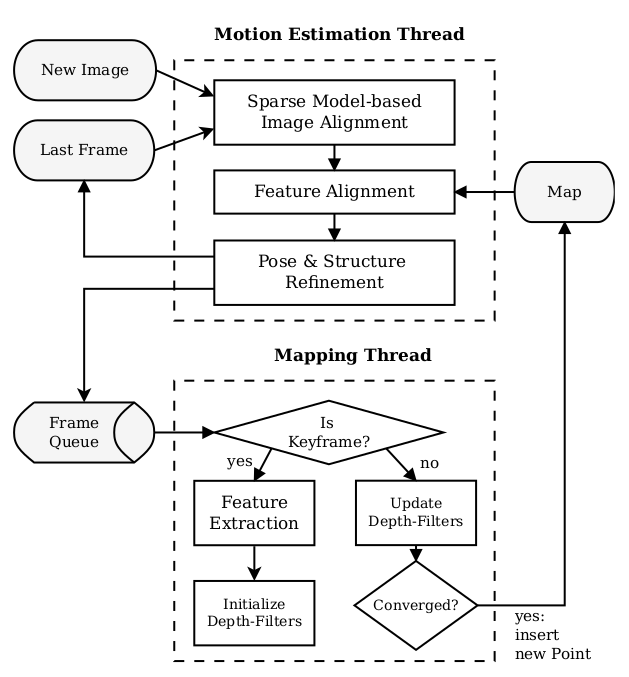
\includegraphics[width=1.0\textwidth]{svo}
	\caption{\acrshort{svo} process overview \cite{Forster2014ICRA}}
	\label{fig:svo}
\end{figure}
\noindent Sparse image alignment estimates the camera pose with respect to previous frame. It always consist some drift which gets accumulated for every next image. Therefore before processing further this relative pose needs to be aligned with respect to 3D map points to reduce the continuous drift. This is further done in feature alignment.
\begin{figure}[h!]
	\centering
	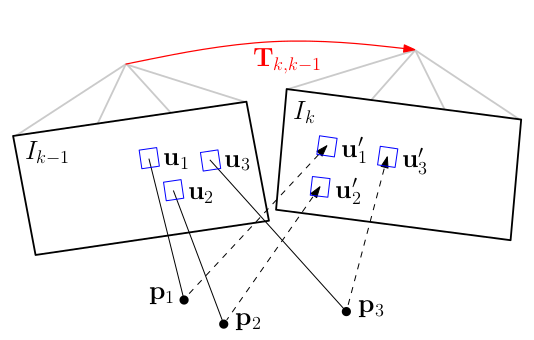
\includegraphics[width=1.0\textwidth]{sparse_img_1}
	\caption{Sparse image alignment minimizes photometric intensity residuals between two image patch (blue squares) corresponding to the same 3D point denoted as $ p_{i}$ \cite{Forster2014ICRA}}
	\label{fig:sparse_img_1}
\end{figure}
\subsubsection{Feature Alignment}
In feature alignment, closest keyframes with respect to current frame are found by checking visibility of 3D keypoints pf that keyframe into current frame. Now, all 3D keypoints from the closest keyframes are projected into the image. For every reprojected points a corresponding 2D point with closest observation angle is found. Then finally it optimizes all 2D points by minimizing photometric error. This problem can be solved using traditional feature tracking method like Lucas-Kanade method \cite{Lucas81}. This step is necessary to reduce drift in camera pose estimated during sparse image alignment. Figure \ref{fig:sparse_img_2}  shows how the 3D map points generated from different keyframes are used to minimize 2D feature point patches in new image.\\
\begin{figure}[H]
	\centering
	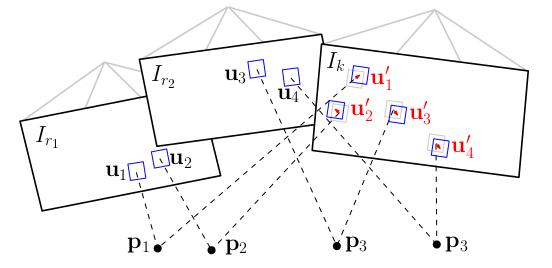
\includegraphics[width=1.0\textwidth]{sparse_img_2}
	\caption{Feature alignment step optimizes corresponding 2D feature patches visible in keyframes $ r_{i} $ and current frame by minimizing photometric error \cite{Forster2014ICRA}.}
	\label{fig:sparse_img_2}
\end{figure}
\noindent Last step in motion estimation thread is pose and structure refinement. Forster et al. found that the reprojection residual is around 0.3 pixels in feature alignment step \cite{Forster2014ICRA}. The final step minimizes this reprojection residuals famously known as motion \acrshort{ba}. It can be solved using Gauss-Newton method which jointly optimizes the camera poses and 3D points in map. \\

\subsubsection{Mapping}
Mapping is an independent thread which estimates the depths of all 2D features from all past frames whose 3D corresponding are unknown. Forster et al. used an slightly different approach than all other methods. They used a probabilistic Bayesian model to update the depth of feature. The Bayesian framework applied in this method is illustrated in figure \ref{fig:depth_filter}. It can be seen that the corresponding point in new frame is always lie on the epipolar line of the frame. The depth can be converted into a 3D point if the variance of distribution is very small. 3D point can be generated using depth and camera intrinsic parameters. \\
\begin{figure}[H]
	\centering
	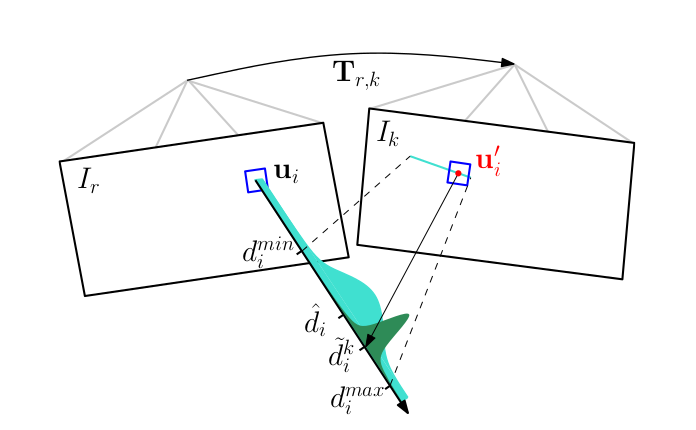
\includegraphics[width=1.0\textwidth]{depth_filter}
	\caption{Probabilistic depth estimate $ d_{i} $ for feature i in the reference frame r. $u_{i} $ is pixels patch surrounding 2D feature \cite{Forster2014ICRA} }
	\label{fig:depth_filter}
\end{figure}
\noindent \acrshort{svo} also uses conditions to consider a frame as keyframe like other \acrshort{vo} methods but in different ways. The one condition is that if camera travels minimum 12\% of average scene depth and if the view is changed 20\% of average scene depth than only a new keyframe is selected. For newly created keyframe, \acrshort{fast} corners are extracted and a depth filter with maximum variance is initiated. The image is divided in cells with fixed size of 30 x 30 pixels and from each cell the corners with highest Shi-Thomasi score are extracted which results in even distribution. These corners are extracted at each level of image pyramid to find best possible corners \cite{Forster2014ICRA}. \\
\newline While for non-keyframes the depth filter associated with reference keyframe is updated by adding the frame and its points(seeds). There is an optional local \acrshort{ba} before adding the frame to depth filter which optimizes all keyframes and its map.\\
\newline After this step old keyframes with farthest distance to the current frame is removed from the map and depth filter simultaneously. On the other hand points with insufficient visibility are removed from depth filter and the points for which epipolar constraint is satisfied with given variance are updated and if converged then its depth is calculated and a new 3D map point is added to the current map which further used in motion estimation thread. Furthermore the converged points (seeds) are removed from depth filter. This mark the end of mapping thread.\\
\newline The depth filter used here has important role in increased speed and accuracy of motion estimation because it generates much less outlier 3D points. It avoids the use of \acrshort{ransac} and further improves the speed. 

